\documentclass[portrait, 25pt, a0paper, blockverticalspace=0.6cm, innermargin=0.6cm, colspace=0.5cm]{tikzposter}\usepackage[]{graphicx}\usepackage[]{color}
% maxwidth is the original width if it is less than linewidth
% otherwise use linewidth (to make sure the graphics do not exceed the margin)
\makeatletter
\def\maxwidth{ %
  \ifdim\Gin@nat@width>\linewidth
    \linewidth
  \else
    \Gin@nat@width
  \fi
}
\makeatother

\definecolor{fgcolor}{rgb}{0.345, 0.345, 0.345}
\newcommand{\hlnum}[1]{\textcolor[rgb]{0.686,0.059,0.569}{#1}}%
\newcommand{\hlstr}[1]{\textcolor[rgb]{0.192,0.494,0.8}{#1}}%
\newcommand{\hlcom}[1]{\textcolor[rgb]{0.678,0.584,0.686}{\textit{#1}}}%
\newcommand{\hlopt}[1]{\textcolor[rgb]{0,0,0}{#1}}%
\newcommand{\hlstd}[1]{\textcolor[rgb]{0.345,0.345,0.345}{#1}}%
\newcommand{\hlkwa}[1]{\textcolor[rgb]{0.161,0.373,0.58}{\textbf{#1}}}%
\newcommand{\hlkwb}[1]{\textcolor[rgb]{0.69,0.353,0.396}{#1}}%
\newcommand{\hlkwc}[1]{\textcolor[rgb]{0.333,0.667,0.333}{#1}}%
\newcommand{\hlkwd}[1]{\textcolor[rgb]{0.737,0.353,0.396}{\textbf{#1}}}%
\let\hlipl\hlkwb

\usepackage{framed}
\makeatletter
\newenvironment{kframe}{%
 \def\at@end@of@kframe{}%
 \ifinner\ifhmode%
  \def\at@end@of@kframe{\end{minipage}}%
  \begin{minipage}{\columnwidth}%
 \fi\fi%
 \def\FrameCommand##1{\hskip\@totalleftmargin \hskip-\fboxsep
 \colorbox{shadecolor}{##1}\hskip-\fboxsep
     % There is no \\@totalrightmargin, so:
     \hskip-\linewidth \hskip-\@totalleftmargin \hskip\columnwidth}%
 \MakeFramed {\advance\hsize-\width
   \@totalleftmargin\z@ \linewidth\hsize
   \@setminipage}}%
 {\par\unskip\endMakeFramed%
 \at@end@of@kframe}
\makeatother

\definecolor{shadecolor}{rgb}{.97, .97, .97}
\definecolor{messagecolor}{rgb}{0, 0, 0}
\definecolor{warningcolor}{rgb}{1, 0, 1}
\definecolor{errorcolor}{rgb}{1, 0, 0}
\newenvironment{knitrout}{}{} % an empty environment to be redefined in TeX

\usepackage{alltt}
\usepackage{url}
\usepackage{graphicx}
\usepackage{booktabs}
\usepackage{adjustbox}
\usepackage{amsmath}
\usepackage{amssymb}
\usepackage{mathtools}
\usepackage{algorithm}
\usepackage{mathtools}
\usepackage{parskip}
\usepackage{tabularx}
\usepackage{natbib}
\usepackage{ngerman}
\usepackage[latin1]{inputenc}
\usepackage[noend]{algpseudocode}
\usepackage[skip=2pt]{caption}
\usepackage{fontawesome}
\DeclareMathOperator*{\argmax}{arg\,max}
\DeclareMathOperator*{\argmin}{arg\,min}
\newcommand{\tdef}{\Theta_{def}}

\definecolor{ao}{rgb}{0.0, 0.45, 0.1}
\definecolor{gainsboro}{rgb}{0.75, 0.75, 0.75}
\definecolor{gainsboro_light}{rgb}{0.93, 0.93, 0.93}
\usecolorstyle[colorOne=white,colorTwo=ao,colorThree=gainsboro]{Britain}
\usetitlestyle[titletotopverticalspace=-10mm,titletoblockverticalspace=-15mm]{Empty}

\title{Multi-Objective AutoML}
\author{
Florian Pfisterer, Janek Thomas, Stefan Coors, Bernd Bischl \\
LMU Munich
}
\IfFileExists{upquote.sty}{\usepackage{upquote}}{}
\begin{document}
\maketitle[width = 0.8\textwidth]


\block[titleinnersep=0.45cm]{Abstract}
{
AutoML systems are currently rising in popularity, as they can build powerful models without human oversight.
They often combine techniques from many different sub-fields of machine learning in order to find a model or set of models that optimize a user-supplied criterion, such as predictive performance. The ultimate goal of such systems is to reduce the amount of time spent on menial tasks, or tasks that can be solved better by algorithms, while leaving decisions that require human intelligence to the end-user. In recent years, the importance of other criteria, such as fairness and interpretability, and many others has become more and more apparent. Current AutoML frameworks either do not allow to optimize such secondary criteria, or only do so by limiting the system's choice of models and preprocessing steps. We propose to optimize additional criteria defined by the user directly to guide the search towards an optimal machine learning pipeline. In order to demonstrate the need and usefulness of our approach, we provide a simple multi-criteria AutoML system and showcase an exemplary application.
}

\begin{columns}
\column{0.5}
  \block[titleinnersep=0.45cm]{TL;DR}
  {
  \centering
  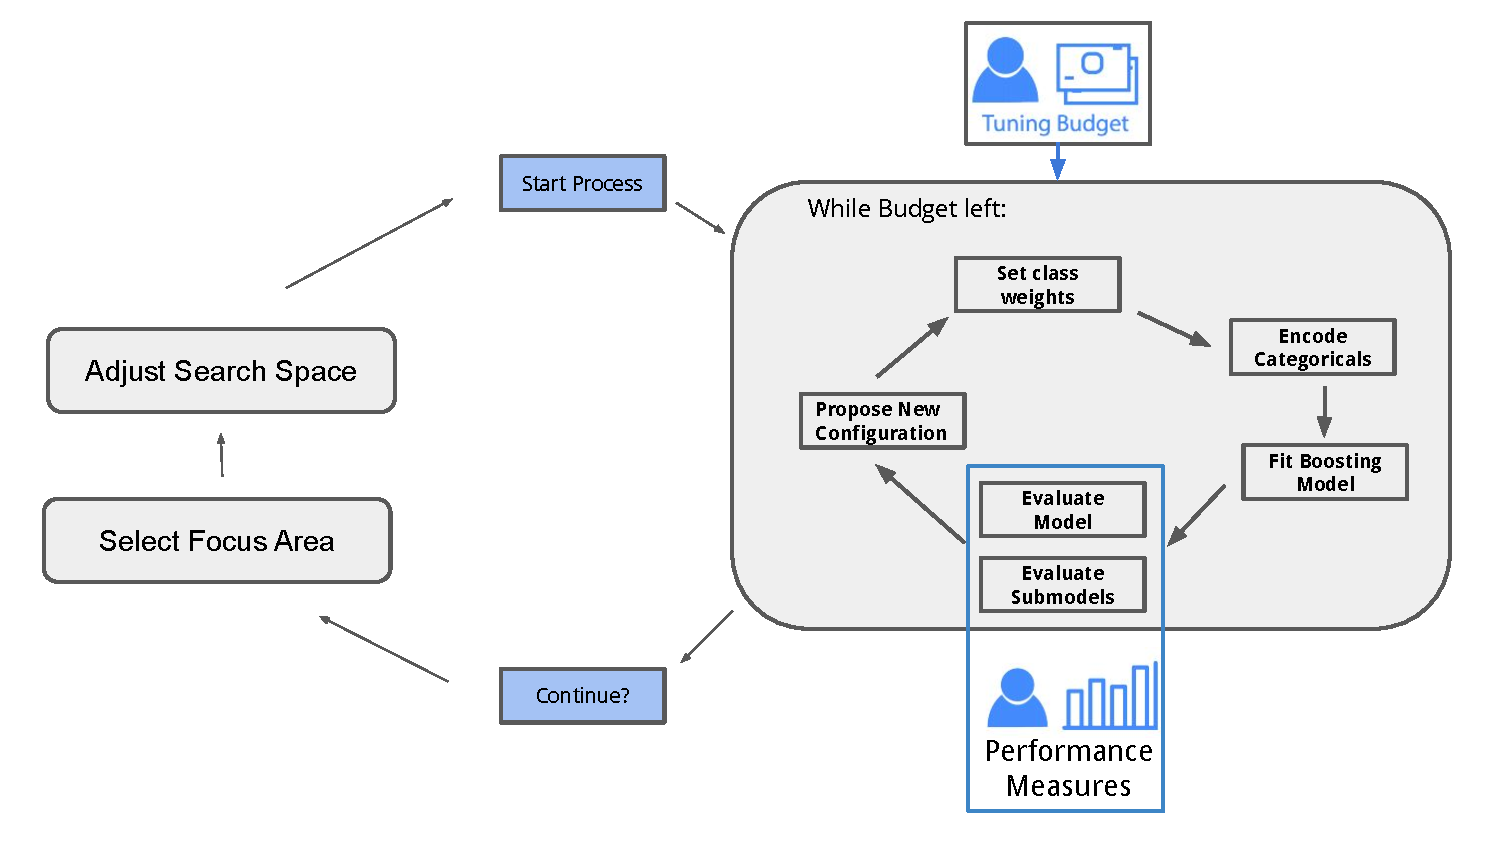
\includegraphics[width=0.42\textwidth]{figures/automl_schema.pdf}

  \innerblock{Problem}{
  \begin{itemize}
    \item Some ML applications require optimizing multiple objectives at the same time.
    \item This is currently not possible in existing AutoML frameworks
    \item Awareness for multiple objectives does also often not exist!
  \end{itemize}
  }
  \vspace{0.4cm}
  \innerblock{Contribution}{
  \begin{itemize}
    \item We provide several interesting measures
    \item We propose a minimalistic implementation of a multi-objective AutoML system
    \item We demonstrate our implementation in a use-case
  \end{itemize}
  }
    \vspace{-.2cm}
  }
  % \block[titleinnersep=0.45cm]{Motivation}
  % {
  % \innerblock{Example 1: Fairness}{
  %   When humans are subject to the decisions of models that are the outcome of AutoML
  %   systems, models need to be \textbf{fair} and yet have a high \textbf{predicitive performance}.
  % }
  % \vspace{1cm}
  % \innerblock{Example 2: Interpretability}{
  %   Regulations might require that the decisions made by models are explainable / interpretable.
  %   As a result, we might only want models that can be interpreted.
  % }
  %  \centering
  %  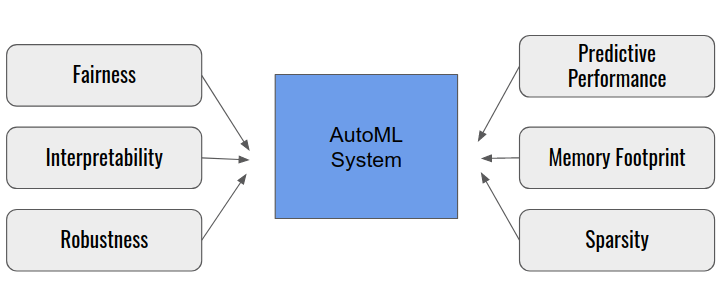
\includegraphics[width=0.4\textwidth]{figures/multicritizzle.png}
  %  \vspace{-0.5cm}
  % }
  \block[titleinnersep=0.45cm]{Measures}
  {
  \innerblock{Fairness}{
  \begin{itemize}
    \item Sufficiency
     \[
    Pr\{Y_b = 1 | A = 0, Y = y\} = Pr\{Y_b = 1 | A = 1, Y = y\}, y \in \{0, 1\}
    \]
    $\rightarrow$ Minimize the absolute difference in FPR, FNR, ... between two sub-populations.
  \end{itemize}
  }

  \innerblock{Interpretability}{
  \begin{itemize}
   \item \textbf{Complexity of main effects} ~\cite{molnar2019quantifying}: Determine shape complexity of ALE main effects by number of parameters needed to approximate the curve with linear segments.

   \item \textbf{Interaction Strength} Impact of interaction effects is relevant when explanations are required,
    as interpretability techniques often use linear relationships to obtain explanations.
    Measures the fraction of variance that can not be explained by main effects.
  \item \textbf{Sparsity} Using fewer features simplifies interpreting models.
  \end{itemize}
  }
    \vspace{0.5cm}
  \innerblock{Robustness}{
  \begin{itemize}
   \item \textbf{Perturbations} Measure classifiers' robustness to perturbations in the input data.
   \item \textbf{Adversarial Examples}
   A variety of robustness measures can be derived from the different types of Adversarial Attacks~\cite{szegedy2013intriguing}
   proposed.
   \item \textbf{Distribution shift} We might want models that are robust or work despite distribution shift.
   How to achieve this is an open research field.
  \end{itemize}
  }
  \vspace{-0.5cm}
  }
\column{0.5}
  \block[titleinnersep=0.45cm]{Method}
  {
  \innerblock{Pipeline}{
  Based on autoxgboost \citep{autoxgboost}, we create a \textbf{single-learner} AutoML system.
  We optimize hyperparameters of xgboost \citep{xgboost} along with class weights, and
  encoding for categorical variables.
  }
  \innerblock{Optimizer}{
  We use Bayesian Optimization with \textbf{parEgo} ~\cite{parego}, as it is a simple method, and it naturally lends itself to focussing on regions
  of the pareto front. \textbf{parEgo} is a rather simple extension, which scalarizes the set of target functions by
  using the augmented Tchebycheff norm
  \[
  \max_{i=1,\dots,k}(w_if_i(\theta)) +\rho\sum_{i=i}^kw_if_i(\theta),
  \]
  with a different uniformly sampled weight vector $w$ such that $\sum_{i=1}^kw_i=1$ in each iteration.
  We can limit the range of projections $w_i$ to focus on certain area's of the pareto front.
  }
  \innerblock{Sub-evaluations}{
    As threshold-tuning and early-stopping are no longer trivial, after each iteration,
    we add different models with $n < nrounds$ and different classification thresholds to the pareto front.
    These can be obtained cheaply for a fixed model.
  }
  \vspace{-.2cm}
  }
  \block[titleinnersep=0.45cm]{Application}
  {
  The Adult dataset contains $48842$ observations of $14$ features, including $6$
  numeric and $8$ factor features describing age, sex, education, marital status, race and more.
  The aim is to predict whether a person's income is below or above 50 k\$ a year.
  We use the mean missclassification error and aim to assure fairness regarding a person's sex.
  We want a model, that performs equally good regardless of which sub-population we are considering.
  As a fairness measure we use the absolute difference in F1-Scores between two sub-populations \textit{male} and \textit{female}.

  \vspace{.4cm}
  \begin{centering}
  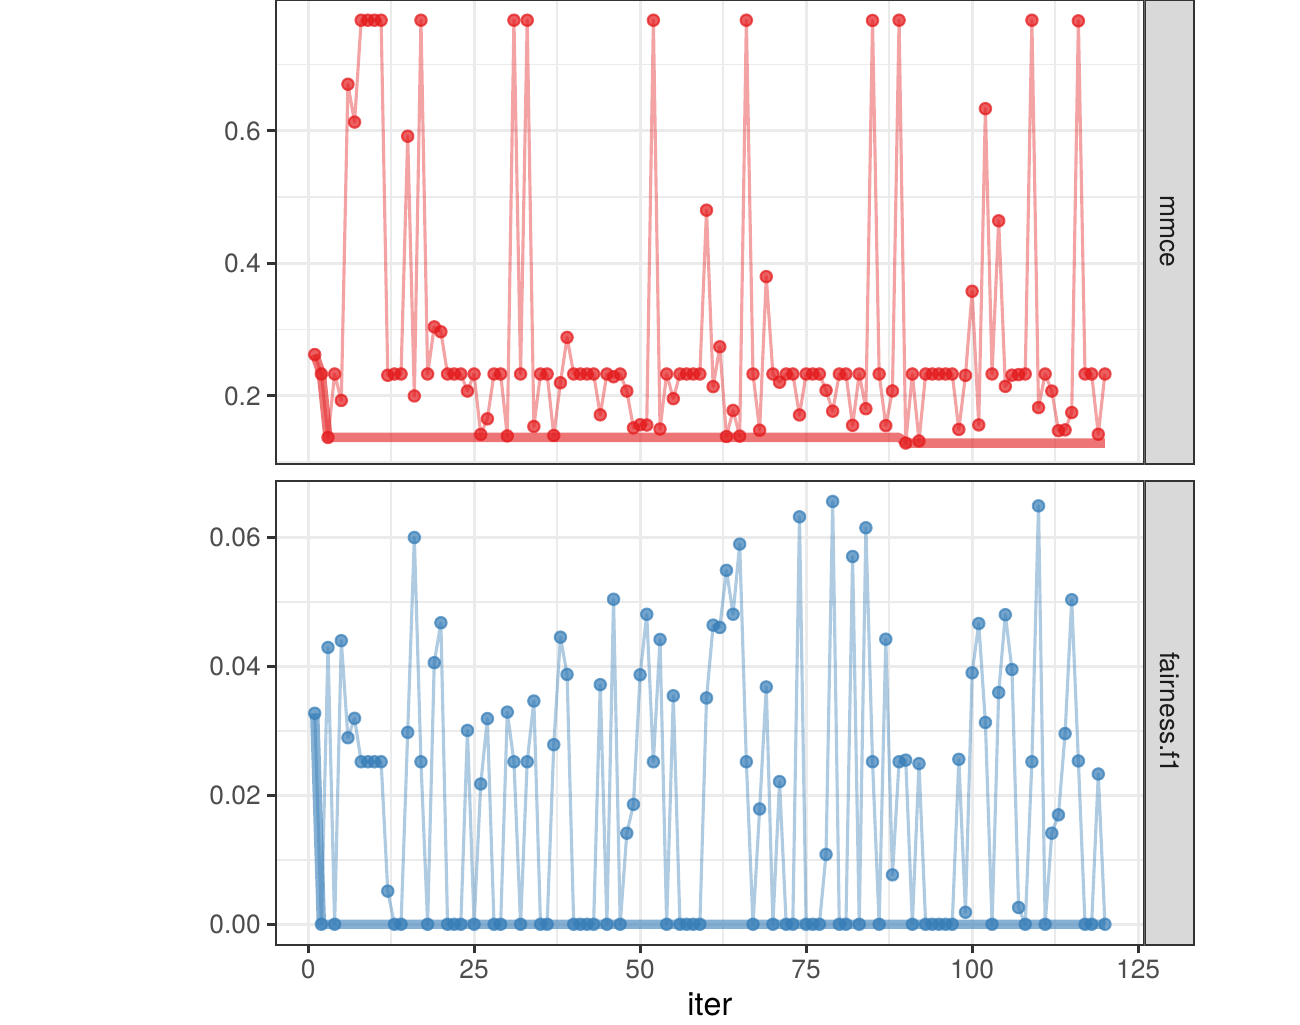
\includegraphics[width=0.8\linewidth]{figures/opt_path.png}

  Tuning progress of the AutoML system on internal validation data.
  \end{centering}
  }
\end{columns}
\begin{columns}

\column{0.35}
  \block[titleinnersep=0.45cm]{References}
    {
    \begingroup
      \renewcommand{\section}[2]{}%
      \small
      \bibliographystyle{plain}
      \bibliography{jmlr-bib}
    \endgroup
    }
\column{0.65}
  \block[titleinnersep=0.45cm]{Application: Pareto Set}{
  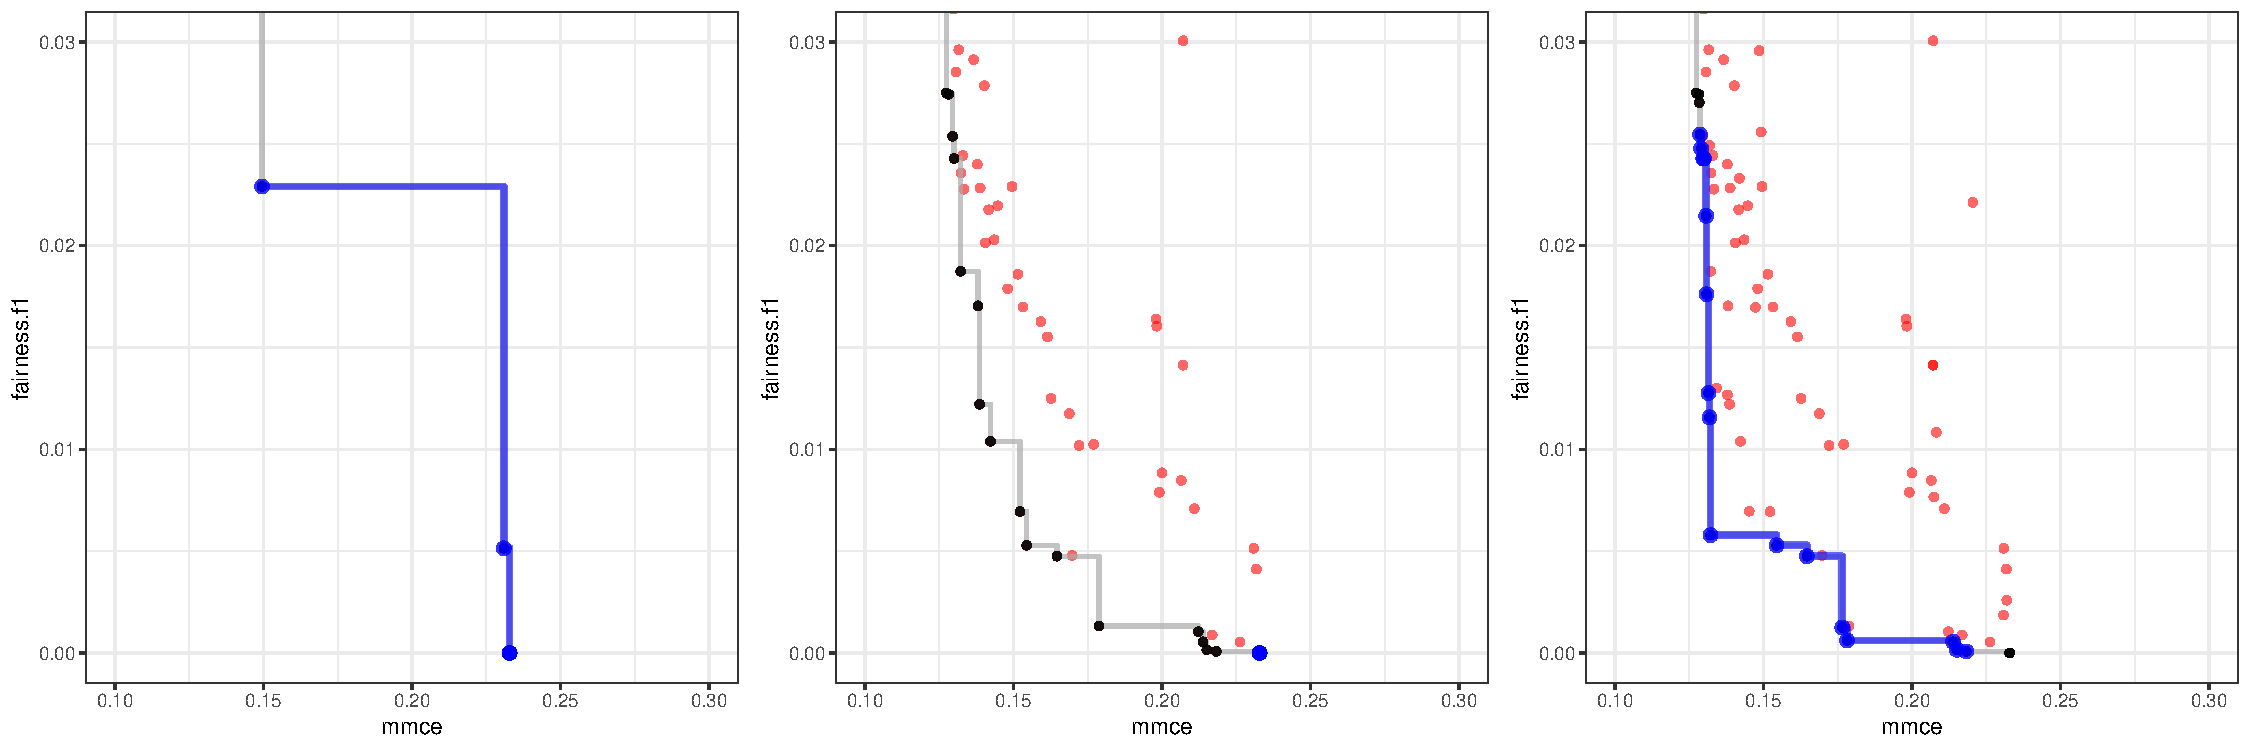
\includegraphics[width=\linewidth]{figures/pareto_plots.pdf}
  Pareto Front after $20$, $70$ and $120$ iterations. Grey line: Pareto front; blue: Focus area
  }
\end{columns}


\block[titleinnersep=0.45cm]{Outlook}
{
\begin{minipage}{0.55\textwidth}
\begin{itemize}
\item Implement pre- and post-processing methods tailored to measures.
\item Add different optimizers (MO-Hyperband, more advanced multi-objective Bayesian Optimization).
\item Explore functionality in different use-cases.
\end{itemize}
\end{minipage}
\begin{minipage}{0.4\textwidth}
  \centering
  \innerblock{Github}{ \faGithub \hspace{.5cm} \url{https://github.com/pfistfl/autoxgboostMC}}
\end{minipage}
}
\nocite{mlr}
\end{document}


